The Fast Adaptive Structured Reporting (FASR) system's goal is to reduce variability and error in radiological interpretation by providing decision-support during reporting time. This works by incorporating multiple checks during the reporting process and providing real-time feedback to the radiologist.

There are three main components to FASR: (1) Verification of the annotation correctness, (2) verification of reporting completeness and (3) providing feedback to the radiologist. In this chapter, we will explain in-depth how FASR solves these tasks.

\begin{figure}[h]
\centering
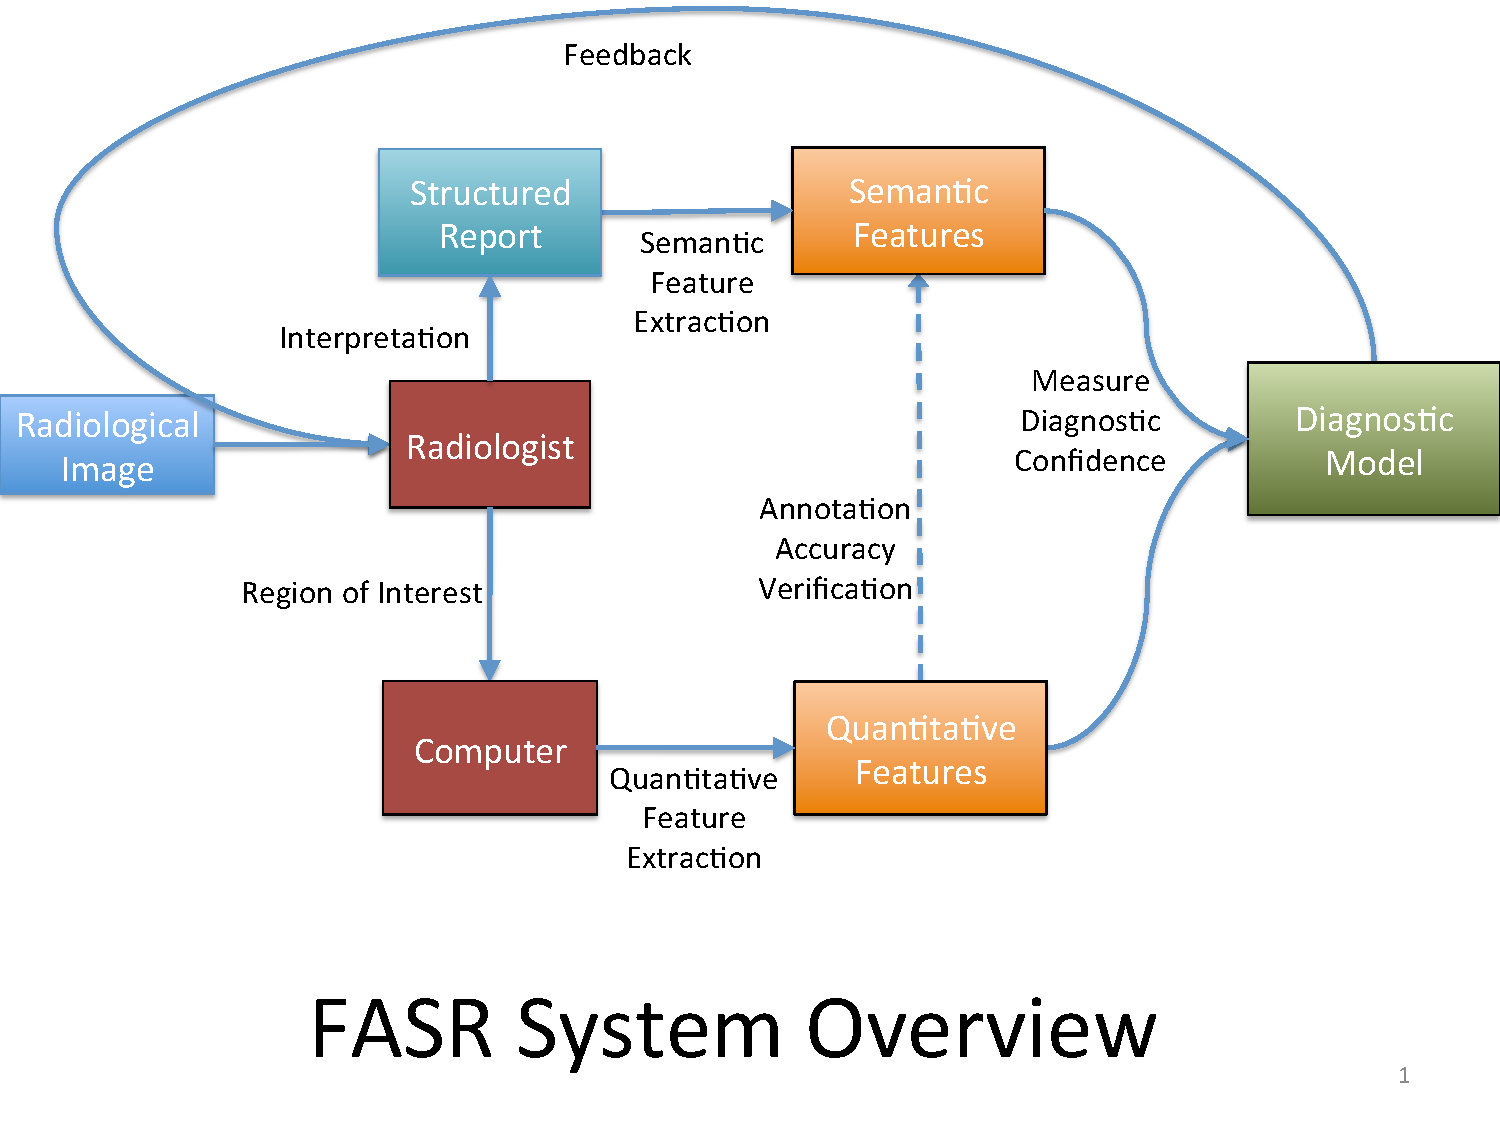
\includegraphics[width=1\linewidth]{fasr_diagram.pdf}
\caption{Overview of the Fast Adaptive Structured Reporting (FASR) system}
\label{fig:fasr_diagram}
\end{figure}